\documentclass[aspectratio=169,11pt]{beamer}

% --- Theme ---
\usetheme{metropolis}
\usepackage{appendixnumberbeamer}

% --- Packages ---
\usepackage{fontspec}
\usepackage{minted}
\setminted{fontsize=\small,breaklines=true}
\usepackage{booktabs}
\usepackage{tikz}
\usepackage{fontawesome5}

% --- Colors ---
\definecolor{healthgreen}{RGB}{34,139,34}
\definecolor{alertred}{RGB}{220,53,69}
\setbeamercolor{alerted text}{fg=alertred}

% --- Metadata ---
\title{Module 10: Capstone project}
\subtitle{Data analysis with Python for health specialists}
\author{Ya\'{e} Ulrich Gaba}
\institute{AIRINA Labs}
\date{2026}

\begin{document}

% ============================================================
\maketitle

% ============================================================
\begin{frame}{The capstone project}
\begin{columns}
\column{0.6\textwidth}
Apply \alert{every skill} from this course to a real health question:
\begin{itemize}
  \item Real public data (no simulated datasets)
  \item Reproducible Jupyter notebook
  \item At least 3 visualizations
  \item At least 1 statistical test or model
  \item Written report (5--8 pages)
  \item 5-minute oral presentation
\end{itemize}

\column{0.35\textwidth}
\centering
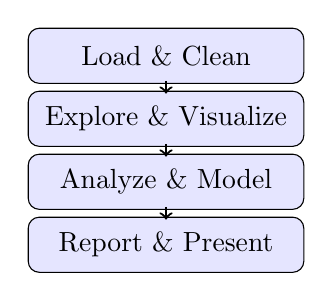
\begin{tikzpicture}[scale=0.8]
\node[draw, rounded corners, fill=blue!10, minimum width=3.5cm, minimum height=0.7cm] at (0, 3) {Load \& Clean};
\node[draw, rounded corners, fill=blue!10, minimum width=3.5cm, minimum height=0.7cm] at (0, 2) {Explore \& Visualize};
\node[draw, rounded corners, fill=blue!10, minimum width=3.5cm, minimum height=0.7cm] at (0, 1) {Analyze \& Model};
\node[draw, rounded corners, fill=blue!10, minimum width=3.5cm, minimum height=0.7cm] at (0, 0) {Report \& Present};
\draw[->, thick] (0, 2.6) -- (0, 2.4);
\draw[->, thick] (0, 1.6) -- (0, 1.4);
\draw[->, thick] (0, 0.6) -- (0, 0.4);
\end{tikzpicture}
\end{columns}
\end{frame}

% ============================================================
\begin{frame}{5 suggested projects}
\begin{table}
\small
\begin{tabular}{clp{6cm}}
\toprule
\textbf{\#} & \textbf{Topic} & \textbf{Key datasets} \\
\midrule
1 & Diabetes risk factors & Pima Indians (UCI), CDC BRFSS \\
2 & COVID-19 across Africa & JHU CSSE, OWID, World Bank \\
3 & Maternal mortality & WHO GHO (MMR, SBA), World Bank, DHS \\
4 & Heart disease prediction & UCI Heart Disease (Cleveland) \\
5 & Malaria burden \& interventions & WHO GHO, Malaria Atlas, DHS \\
\bottomrule
\end{tabular}
\end{table}

\vspace{6pt}
You may also \textbf{propose your own project} (subject to instructor approval).
\end{frame}

% ============================================================
\begin{frame}{Project 1: Diabetes risk factors}
\textbf{Objective:} Identify strongest risk factors and build a predictive model.

\vspace{4pt}
\textbf{Required analyses:}
\begin{enumerate}
  \item Clean Pima dataset (handle zeros as missing)
  \item EDA: distributions, correlations, box plots by diabetes status
  \item Logistic regression: odds ratios with 95\% CIs
  \item Compare logistic regression vs.\ random forest (accuracy, AUC-ROC)
\end{enumerate}

\textbf{Deliverables:} correlation heatmap, ROC curves, OR table, clinical interpretation.
\end{frame}

% ============================================================
\begin{frame}{Project 2: COVID-19 impact in Africa}
\textbf{Objective:} Analyze differential COVID-19 impact and correlations with health system capacity.

\vspace{4pt}
\textbf{Required analyses:}
\begin{enumerate}
  \item Select 10--15 African countries across subregions
  \item Epidemic curves (7-day rolling average), identify wave patterns
  \item Key metrics: cases/million, deaths/million, CFR, vaccination rate
  \item Merge with World Bank indicators; correlations with health expenditure
  \item Choropleth map of case fatality rates
\end{enumerate}

\textbf{Deliverables:} epi curves, scatter plots, choropleth, summary table.
\end{frame}

% ============================================================
\begin{frame}{Project 3: Maternal mortality determinants}
\textbf{Objective:} Which health system and socioeconomic factors predict MMR?

\vspace{4pt}
\textbf{Required analyses:}
\begin{enumerate}
  \item Load WHO GHO MMR data; identify 20 worst countries
  \item Merge with skilled birth attendance, antenatal care, GDP, female literacy
  \item Scatter plots + Pearson/Spearman correlations
  \item Multiple linear regression predicting MMR; check assumptions
  \item Choropleth map of MMR across Africa
\end{enumerate}

\textbf{Deliverables:} scatter plots with regression lines, regression table, choropleth, policy discussion.
\end{frame}

% ============================================================
\begin{frame}{Projects 4 \& 5}
\textbf{Project 4 --- Heart disease prediction:}
\begin{itemize}
  \item Compare 4 models (logistic, decision tree, random forest, KNN)
  \item ROC curves on one figure, confusion matrix, feature importance
  \item Clinical interpretation: do top predictors match cardiology guidelines?
\end{itemize}

\vspace{8pt}
\textbf{Project 5 --- Malaria burden \& interventions:}
\begin{itemize}
  \item Incidence trends (2000--2022) for 10 high-burden countries
  \item Correlate changes in ITN use / IRS coverage with incidence decline
  \item Choropleth of current malaria incidence
  \item Regression: does intervention coverage predict incidence change?
\end{itemize}
\end{frame}

% ============================================================
\begin{frame}{Report template}
\begin{enumerate}
  \item \textbf{Introduction} (0.5--1 page): health context, research question, dataset overview
  \item \textbf{Data description} (1 page): source, variables, summary stats, missing data handling
  \item \textbf{Methods} (1 page): cleaning steps, tests/models chosen and why, validation strategy
  \item \textbf{Results} (1.5--2 pages): figures, tables, test statistics, model metrics
  \item \textbf{Discussion} (1--1.5 pages): clinical meaning, comparison with literature, implications
  \item \textbf{Limitations} (0.5 page): data quality, generalizability, future work
\end{enumerate}

\begin{alertblock}{Figures rule}
Every figure must have a title, labeled axes, and a caption. Figures without labels = lost marks.
\end{alertblock}
\end{frame}

% ============================================================
\begin{frame}{Grading rubric}
\begin{table}
\begin{tabular}{lc}
\toprule
\textbf{Component} & \textbf{Points} \\
\midrule
Research question & 10 \\
Data handling (loading, cleaning, documentation) & 15 \\
Exploratory analysis (stats + 3 visualizations) & 15 \\
Statistical analysis / modeling & 20 \\
Report quality (writing, figures, limitations) & 20 \\
Code quality (reproducible, commented) & 10 \\
Oral presentation (5 min, answers questions) & 10 \\
\midrule
\textbf{Total} & \textbf{100} \\
\bottomrule
\end{tabular}
\end{table}
\end{frame}

% ============================================================
\begin{frame}{Presentation guidelines}
\textbf{5 minutes + 2--3 min questions.} Structure:
\begin{enumerate}
  \item \textbf{Slide 1:} Title, your name, date
  \item \textbf{Slide 2:} Motivation --- why does this health question matter?
  \item \textbf{Slide 3:} Data --- source, $n$, key variables
  \item \textbf{Slides 4--5:} Key results --- your 2--3 best figures
  \item \textbf{Slide 6:} Conclusions --- 1--2 take-home messages
\end{enumerate}

\vspace{6pt}
\textbf{Tips:} One message per slide. No code on slides. Speak to the audience, not the screen. Practice with a timer.
\end{frame}

% ============================================================
\begin{frame}[fragile]{Today: get started}
\textbf{Complete this checklist before you leave:}
\begin{enumerate}
  \item Choose your project (1--5 or custom)
  \item Download dataset, run \texttt{.head()} and \texttt{.shape}
  \item Write your research question in one sentence
  \item List 3 planned visualizations and 1 statistical test
  \item Identify potential data problems
  \item Create your project folder:
\begin{minted}{text}
capstone_project/
    data/raw/
    data/cleaned/
    notebooks/
    figures/
    report.pdf
\end{minted}
\end{enumerate}
\end{frame}

% ============================================================
\begin{frame}{Timeline}
\begin{table}
\begin{tabular}{lp{9cm}}
\toprule
\textbf{Week} & \textbf{Milestone} \\
\midrule
Week 1 & Choose project, download data, initial exploration \\
Week 2 & Complete analysis, generate figures/tables, draft report \\
Week 3 & Finalize report, prepare and deliver 5-minute presentation \\
\bottomrule
\end{tabular}
\end{table}

\vspace{12pt}
\centering
\Large \faIcon{rocket} \alert{You have all the skills. Now apply them.}
\end{frame}

% ============================================================
\begin{frame}{Exercises (Hour 3)}
\begin{enumerate}
  \item \textbf{Pair review:} Present your research question and initial data exploration to a partner; give and receive feedback
  \item \textbf{Data check:} Verify your dataset loads correctly, identify missing values, and plan your cleaning steps
  \item \textbf{Analysis plan:} Write a 1-paragraph plan describing your 3 visualizations and 1 model/test
  \item \textbf{Submit:} Project choice + research question to the instructor by end of session
\end{enumerate}
\end{frame}

\end{document}
